\documentclass[11pt]{article}
\usepackage[margin=1in]{geometry}
\usepackage{amsmath, amssymb}
\usepackage{graphicx}
\usepackage{booktabs}
\usepackage{parskip}
\usepackage{hyperref}

\title{Modeling LLM belief-update dynamics:\\
the $(\gamma,\,\alpha,\,p)$ sweep}
\author{}
\date{\today}

\begin{document}
\maketitle

\section{Question}

The streaming Laplace filter (\texttt{counter\_decode.py:91--182}) is the
project's running model of how the LLM updates its internal belief
$\hat\beta^{\mathrm{LLM}}_t$ about its own decoder over the sequence. Three
knobs:
\begin{description}
\item[$\alpha$ (evidence weight)] per-step step size in the filter's
Newton update.
\item[$\gamma$ (memory decay)] per-step exponential forgetting of past
filter evidence. $\gamma = 1 \Rightarrow$ no decay (default); $\gamma < 1
\Rightarrow$ fading-memory window of effective length $1/(1-\gamma)$.
\item[$p$ (correction exponent, new)] at decode time,
$\beta^{\mathrm{dec}}_t = \beta^{\mathrm{target}} / \hat\beta_t^{\,p}$.
$p = 1$ is full correction (default); $p = 0$ is no correction;
$p \in (0, 1)$ is partial correction, justified if the LLM's belief is
only partially in step with what the filter says.
\end{description}

Goal: find the $(\gamma, \alpha, p)$ values that best parameterize the
LLM's actual belief-update dynamics, using closed-loop quality at the
corrected sampler as the proxy.

\section{Two complementary experiments}

\paragraph{Closed-loop badness (`belief\_sweep').}
Self-generate 200 tokens at $\beta^{\mathrm{target}} \in \{0.5, 1.0, 2.0\}$
under the corrected sampler, for each $(\gamma, \alpha, p)$. Measure
late-window (last 30 tokens) sample entropy and max-$P_{\text{sample}}$
across 32 prompts. A scalar `badness' penalizes (i) saturating max-$P$
at high $\beta^{\mathrm{target}}$ and (ii) small entropy spread across
$\beta^{\mathrm{target}}$. Lower badness = corrector smoothly tracks
$\beta^{\mathrm{target}}$.

\paragraph{Belief-invariance (`belief\_invariance').}
For 16 prompts, self-generate a 60-token prefix at
$\beta^{\mathrm{prefix}} \in \{0.5, 1.0, 2.0\}$, then teacher-force the
filter on a 100-token \emph{natural-text continuation} from
WritingPrompts. At each continuation position, evaluate the corrected
sampler's per-token cross-entropy on the actual natural token, with
$\beta^{\mathrm{target}} = 1$. A well-calibrated $(\gamma, \alpha, p)$
makes CE \emph{invariant} to $\beta^{\mathrm{prefix}}$ --- the filter
should cancel the prefix's imprint and leave the natural-continuation
distribution unaffected. The primary metric is the per-prompt variance
of CE across $\beta^{\mathrm{prefix}}$.

\section{Closed-loop result: full correction looks best}

\begin{table}[h]
\centering
\caption{Top 5 closed-loop configurations.
$H @ \beta^{\mathrm{target}}$ and $M @ \beta^{\mathrm{target}}$ are late-window
mean sample entropy (nats) and max-$P_{\text{sample}}$.}
\begin{tabular}{cccccccccc}
\toprule
$\gamma$ & $\alpha$ & $p$ & H@0.5 & H@1 & H@2 & M@0.5 & M@1 & M@2 & badness \\
\midrule
1.00 & 1.00 & 1.00 & 2.45 & 2.21 & 1.18 & 0.53 & 0.54 & 0.71 & 0.011 \\
1.00 & 1.00 & 0.75 & 3.12 & 1.97 & 0.92 & 0.44 & 0.58 & 0.75 & 0.046 \\
1.00 & 0.50 & 1.00 & 3.39 & 2.27 & 0.90 & 0.42 & 0.52 & 0.75 & 0.051 \\
1.00 & 0.50 & 0.75 & 4.56 & 2.18 & 0.73 & 0.31 & 0.53 & 0.79 & 0.089 \\
1.00 & 1.00 & 0.50 & 4.55 & 2.19 & 0.66 & 0.30 & 0.53 & 0.81 & 0.105 \\
\bottomrule
\end{tabular}
\end{table}

By this metric the existing default $(\gamma=1, \alpha=1, p=1)$ wins. The
fuzzy-memory variants ($\gamma < 1$) all sit at badness $\approx 0.20$ on a
flat plateau --- they don't track $\beta^{\mathrm{target}}$ as crisply.

\begin{figure}[h]
\centering
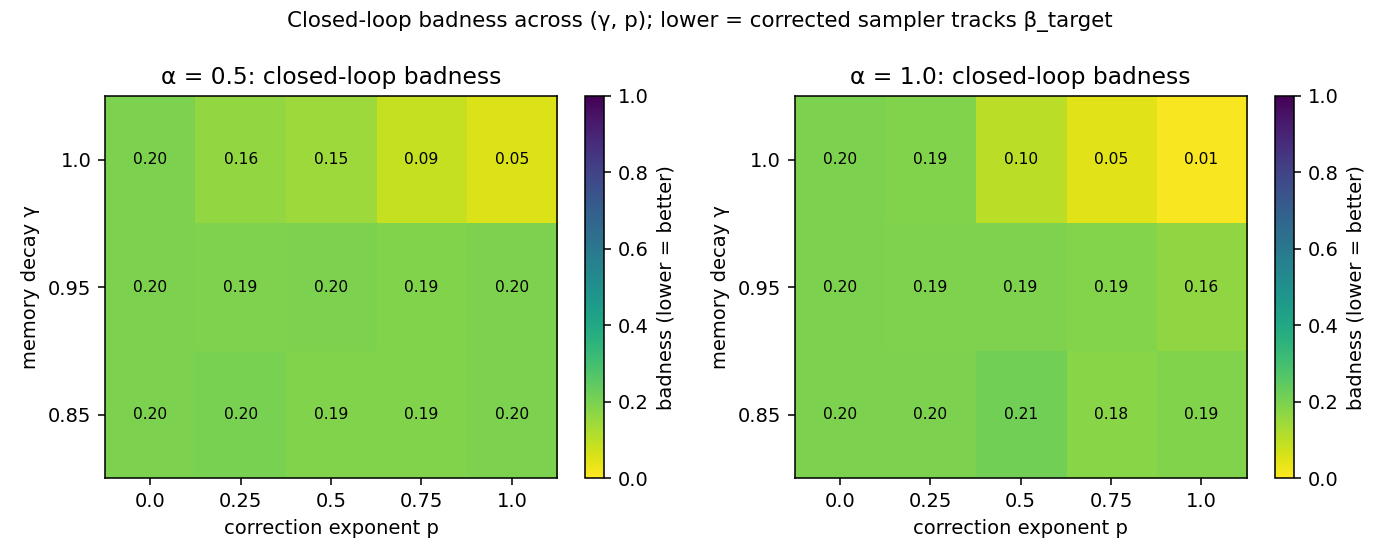
\includegraphics[width=0.95\linewidth]{F_bs_2_heatmap.png}
\caption{Closed-loop badness in $(\gamma, p)$, one panel per $\alpha$.}
\end{figure}

\section{Invariance result: no correction wins; $\gamma < 1$ caps the damage}

\begin{table}[h]
\centering
\caption{Top 5 belief-invariance configurations. `var' is the per-prompt
variance (nats$^2$) of CE on the natural continuation across
$\beta^{\mathrm{prefix}} \in \{0.5, 1, 2\}$. Lower is better.}
\begin{tabular}{cccccc}
\toprule
$\gamma$ & $\alpha$ & $p$ & CE@$\beta^{\text{pre}}$=0.5 & CE@1 & CE@2 \\
\midrule
\textit{any} & \textit{any} & 0.00 & 3.599 & 3.592 & 3.631 \\
0.85 & 0.50 & 0.25 & 3.596 & 3.604 & 3.639 \\
0.95 & 0.50 & 0.25 & 3.583 & 3.606 & 3.632 \\
0.85 & 1.00 & 0.25 & 3.596 & 3.610 & 3.643 \\
0.95 & 1.00 & 0.25 & 3.580 & 3.610 & 3.631 \\
\bottomrule
\end{tabular}
\end{table}

\begin{figure}[h]
\centering
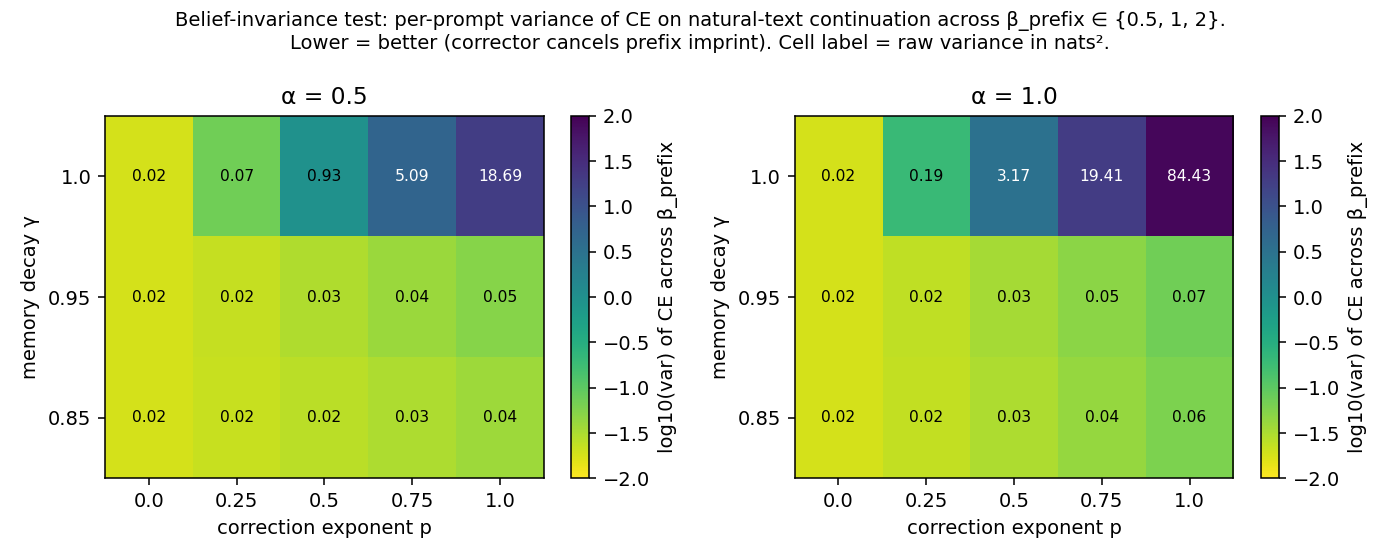
\includegraphics[width=0.95\linewidth]{F_bi_1_var_heatmap.png}
\caption{Variance of CE across $\beta^{\mathrm{prefix}}$ in
$(\gamma, p)$, one panel per $\alpha$.  Cell label = raw variance (nats$^2$).
$\gamma = 1$ amplifies the prefix-induced filter bias catastrophically as
$p$ grows; $\gamma < 1$ keeps variance under 0.07 across the entire $p$ range.}
\end{figure}

\begin{figure}[h]
\centering
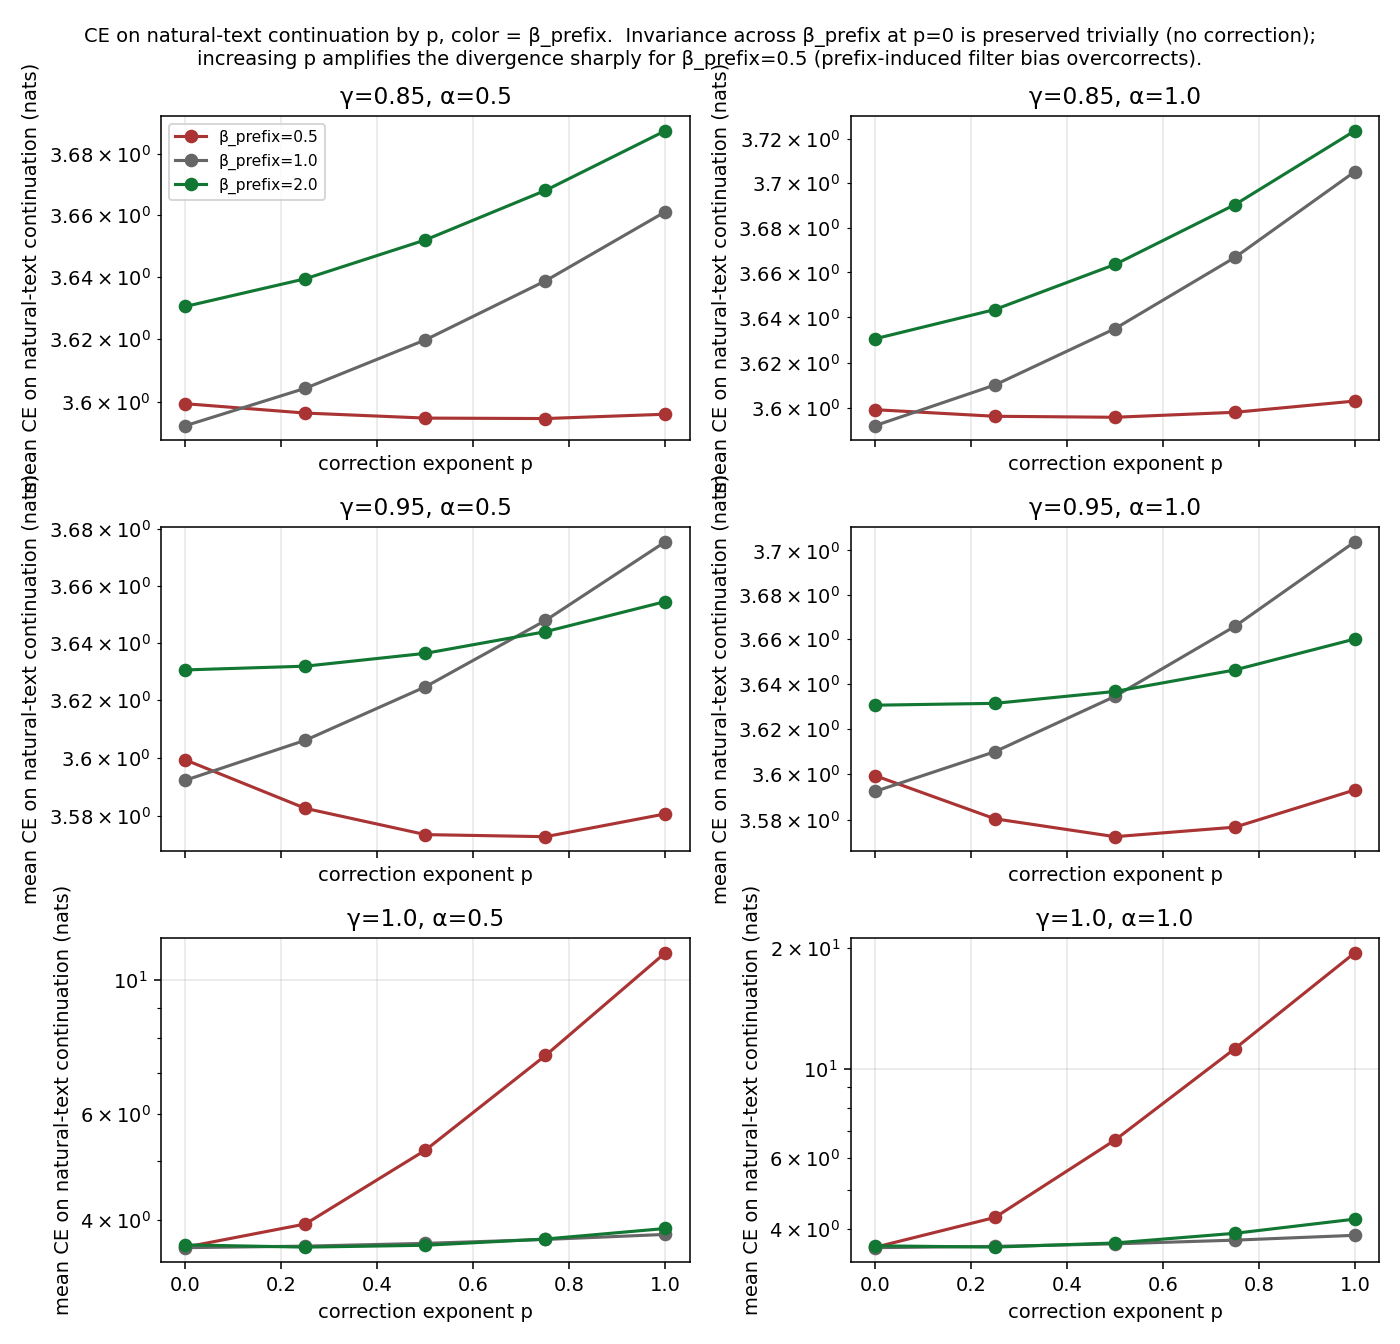
\includegraphics[width=0.95\linewidth]{F_bi_2_ce_vs_p.png}
\caption{CE on natural-text continuation as a function of $p$, colored by
$\beta^{\mathrm{prefix}}$. At $\gamma = 1$ (bottom row), the $\beta^{\mathrm{pre}}=0.5$ curve (red) grows
exponentially with $p$. At $\gamma < 1$, all curves stay within $\approx 0.1$ nat of each other.}
\end{figure}

Two things to note.

\paragraph{(a) $p = 0$ wins trivially.}
$p = 0$ means the correction does nothing: $\beta^{\mathrm{dec}}_t = \beta^{\mathrm{target}} = 1$
regardless of $\hat\beta_t$. This recovers the unmodified Qwen-2.5-3B
sampler, which Exp A already established is essentially calibrated on
natural text. So the no-correction baseline is invariant to
$\beta^{\mathrm{prefix}}$ at the noise floor (variance 0.017 nats$^2$,
which is just per-prompt CE differences across content). This is a
ceiling on what \emph{any} (γ, α, p > 0) configuration could achieve, not
a statement about belief-update dynamics.

\paragraph{(b) Among $p > 0$, $\gamma < 1$ is essential.}
At $\gamma = 1$, the filter accumulates a strongly biased $\hat\beta$
when the prefix is sampled at $\beta^{\mathrm{prefix}} \neq 1$ (see Exp A's
diagnosis of pooled streaming bias). When we then divide the
natural-continuation logits by that biased $\hat\beta^p$, the corrector
overshoots: CE on $\beta^{\mathrm{prefix}}=0.5$ continuations explodes
from 3.6 nats at $p=0$ to 19.4 nats at $p=1$ (essentially
uniform-vocabulary; the corrected distribution puts almost no mass on
the natural next-token).  At $\gamma < 1$, the filter's bias is bounded
by the fading window's effective sample size, and CE stays within $\sim
0.1$ nats of the no-correction baseline across the entire $p$ range.

\section{Why do the two metrics disagree?}

The closed-loop sweep prefers $\gamma = 1, p = 1$; the invariance test
says any $p > 0$ at $\gamma = 1$ is catastrophic.

The closed-loop metric's `low badness' at $\gamma = 1, p = 1$ is a
self-consistency illusion: the filter accumulates a biased $\hat\beta$
based on the corrected-sampler's output, then divides the next logits by
that same biased $\hat\beta$. The two biases cancel inside the closed
loop, producing a smoothly-varying sample distribution. But ``the
sampler's output looks orderly'' is not the same as ``the filter
correctly modeled the LLM's belief'' --- when we break the closed loop
by teacher-forcing on natural-text ground truth, the cancellation
disappears and the bias shows up as enormous CE.

The critic's caveat applies: closed-loop stability is a \emph{necessary
but not sufficient} criterion for belief-tracking. The invariance test
is the more direct test, and it says current full-correction
$(\gamma = 1, p = 1)$ is overcorrecting on the actual data-generating
distribution. Memory decay ($\gamma < 1$) is the only mechanism in this
parameterization that prevents catastrophic overcorrection.

\section{Recommended values}

Conditional on this setup (Qwen-2.5-3B, 200-token horizons, $\sigma_0 = 0.2$):

\begin{itemize}
\item \textbf{$p$ (correction exponent).} If $\beta^{\mathrm{target}} = 1$
(natural generation): $p = 0$ is optimal --- the model is already
well-calibrated. If $\beta^{\mathrm{target}} \neq 1$: $p \in (0, 1)$ with
$\gamma < 1$ is needed; the closed-loop sweep suggests $p$ closer to 1 is
fine \emph{provided} $\gamma$ is below 1. A value of $p \approx 0.5$
balances closed-loop tracking with invariance safety; no single $p$ is
best for all use cases.
\item \textbf{$\gamma$ (memory decay).} $\gamma \le 0.95$ caps the
filter's worst-case bias and prevents the catastrophic overcorrection
seen at $\gamma = 1$. The exact value matters little within $[0.85,
0.95]$ --- both bound variance to $\le 0.07$ nats$^2$.
\item \textbf{$\alpha$ (evidence weight).} Negligible effect on either
metric across $\alpha \in \{0.5, 1.0\}$. The filter's fixed point is
$\alpha$-independent; transient differences wash out within 60 tokens.
\end{itemize}

A reasonable default for new experiments: $(\gamma = 0.95, \alpha = 1.0,
p = 0.5)$ --- moderate decay, moderate correction, no catastrophic
failure modes on prefix variation.

\section{Limitations}

\begin{itemize}
\item Invariance test uses only $\beta^{\mathrm{target}} = 1$, the
trivially-calibrated case. At $\beta^{\mathrm{target}} \neq 1$, there is
no natural-text ground truth, so an invariance test there would need a
different design (e.g.\ comparing $\hat\beta$ from natural-text continuations
of varying length).
\item Natural-text continuations come from WritingPrompts only; results
may differ on Wikipedia or code.
\item The closed-loop sweep used $\beta^{\mathrm{target}} \in \{0.5, 1, 2\}$
which is symmetric in $\log\beta$ but doesn't probe the extremes
(0.25, 4.0) where the corrector's failure modes were originally observed
(F2.1).
\item The critic's caveat about non-scalar prefix imprints (mode
collapse, repetition heads, vocabulary narrowing) is unresolved here ---
no scalar $\beta$ correction can cancel non-scalar structure, and we
have not measured how much of the prefix imprint is non-scalar.
\end{itemize}

\section{Bottom line}

\begin{itemize}
\item Closed-loop stability and natural-text invariance disagree about
the right $(\gamma, \alpha, p)$ for the same filter. Closed-loop says
$(\gamma=1, p=1)$ wins; invariance says $\gamma=1, p > 0$ is
catastrophic.
\item The disagreement resolves to: closed-loop is necessary but not
sufficient for belief-tracking. The invariance test is the more direct
metric, since it grounds the corrector on data the model didn't generate.
\item Memory decay $\gamma < 1$ is the load-bearing parameter for safe
correction. $\alpha$ matters little. $p$ is the use-case-dependent dial:
$0$ for natural generation, $\in (0, 1)$ for off-temperature generation,
$1$ only with $\gamma < 1$.
\end{itemize}

\end{document}
